% !TEX TS-program = XeLaTeX
% use the following command:
% all document files must be coded in UTF-8
\documentclass[english]{textolivre}
% build HTML with: make4ht -e build.lua -c textolivre.cfg -x -u article "fn-in,svg,pic-align"

\journalname{Texto Livre}
\thevolume{19}
%\thenumber{1} % old template
\theyear{2026}
\receiveddate{\DTMdisplaydate{2026}{1}{1}{-1}} % YYYY MM DD
\accepteddate{\DTMdisplaydate{2026}{2}{12}{-1}}
\publisheddate{\DTMdisplaydate{2026}{6}{15}{-1}}
\corrauthor{Diana Ruiz-Onofre}
\articledoi{10.1590/1983-3652.2026.63708}
%\articleid{NNNN} % if the article ID is not the last 5 numbers of its DOI, provide it using \articleid{} commmand 
% list of available sesscions in the journal: articles, dossier, reports, essays, reviews, interviews, editorial
\articlesessionname{articles}
\runningauthor{Moreno-Gudiño and Ruiz-Onofre} 
%\editorname{Leonardo Araújo} % old template
\sectioneditorname{Daniervelin Pereira~\orcid{0000-0003-1861-3609}}
\layouteditorname{Leonardo Araujo~\orcid{0000-0003-3884-2177}}

\title{Digital fragility and academic continuity: the impact of the 2024 energy crisis on hybrid higher education in Ecuador}
\othertitle{Fragilidade digital e continuidade acadêmica: o impacto da crise energética de 2024 na educação superior híbrida no Equador}
% if there is a third language title, add here:
%\othertitle{Artikelvorlage zur Einreichung beim Texto Livre Journal}

\author[1]{Patricio Moreno-Gudiño~\orcid{0000-0002-3184-4965}\thanks{Email: \href{mailto:bpmoreno1@espe.edu.ec}{bpmoreno1@espe.edu.ec}}}
\author[2]{Diana Ruiz-Onofre~\orcid{0000-0002-7121-1548}\thanks{Email: \href{mailto:caridad.ruiz@upec.edu.ec}{caridad.ruiz@upec.edu.ec}}}
\affil[1]{Universidad de las Fuerzas Armadas, Unidad de
Admisión, Sangolquí, Ecuador.}
\affil[2]{Universidad Politécnica Estatal del Carchi, Facultad de Ciencias de la Salud y Ciencias de la Educación, Carrera de Educación Básica, Tulcán, Ecuador.}

\addbibresource{article.bib}
% use biber instead of bibtex
% $ biber article

% used to create dummy text for the template file
\definecolor{dark-gray}{gray}{0.35} % color used to display dummy texts
\usepackage{lipsum}
\SetLipsumParListSurrounders{\colorlet{oldcolor}{.}\color{dark-gray}}{\color{oldcolor}}

% used here only to provide the XeLaTeX and BibTeX logos
\usepackage{hologo}

% if you use multirows in a table, include the multirow package
\usepackage{multirow}

% provides sidewaysfigure environment
\usepackage{rotating}

% CUSTOM EPIGRAPH - BEGIN 
%%% https://tex.stackexchange.com/questions/193178/specific-epigraph-style
\usepackage{epigraph}
\renewcommand\textflush{flushright}
\makeatletter
\newlength\epitextskip
\pretocmd{\@epitext}{\em}{}{}
\apptocmd{\@epitext}{\em}{}{}
\patchcmd{\epigraph}{\@epitext{#1}\\}{\@epitext{#1}\\[\epitextskip]}{}{}
\makeatother
\setlength\epigraphrule{0pt}
\setlength\epitextskip{0.5ex}
\setlength\epigraphwidth{.7\textwidth}
% CUSTOM EPIGRAPH - END

% to use IPA symbols in unicode add
%\usepackage{fontspec}
%\newfontfamily\ipafont{CMU Serif}
%\newcommand{\ipa}[1]{{\ipafont #1}}
% and in the text you may use the \ipa{...} command passing the symbols in unicode

% LANGUAGE - BEGIN
% ARABIC
% for languages that use special fonts, you must provide the typeface that will be used
% \setotherlanguage{arabic}
% \newfontfamily\arabicfont[Script=Arabic]{Amiri}
% \newfontfamily\arabicfontsf[Script=Arabic]{Amiri}
% \newfontfamily\arabicfonttt[Script=Arabic]{Amiri}
%
% in the article, to add arabic text use: \textlang{arabic}{ ... }
%
% RUSSIAN
% for russian text we also need to define fonts with support for Cyrillic script
% \usepackage{fontspec}
% \setotherlanguage{russian}
% \newfontfamily\cyrillicfont{Times New Roman}
% \newfontfamily\cyrillicfontsf{Times New Roman}[Script=Cyrillic]
% \newfontfamily\cyrillicfonttt{Times New Roman}[Script=Cyrillic]
%
% in the text use \begin{russian} ... \end{russian}
% LANGUAGE - END

% EMOJIS - BEGIN
% to use emoticons in your manuscript
% https://stackoverflow.com/questions/190145/how-to-insert-emoticons-in-latex/57076064
% using font Symbola, which has full support
% the font may be downloaded at:
% https://dn-works.com/ufas/
% add to preamble:
% \newfontfamily\Symbola{Symbola}
% in the text use:
% {\Symbola }
% EMOJIS - END

% LABEL REFERENCE TO DESCRIPTIVE LIST - BEGIN
% reference itens in a descriptive list using their labels instead of numbers
% insert the code below in the preambule:
%\makeatletter
%\let\orgdescriptionlabel\descriptionlabel
%\renewcommand*{\descriptionlabel}[1]{%
%  \let\orglabel\label
%  \let\label\@gobble
%  \phantomsection
%  \edef\@currentlabel{#1\unskip}%
%  \let\label\orglabel
%  \orgdescriptionlabel{#1}%
%}
%\makeatother
%
% in your document, use as illustraded here:
%\begin{description}
%  \item[first\label{itm1}] this is only an example;
%  % ...  add more items
%\end{description}
% LABEL REFERENCE TO DESCRIPTIVE LIST - END


% add line numbers for submission
%\usepackage{lineno}
%\linenumbers

\begin{document}
\maketitle

\begin{polyabstract}
\begin{abstract}
This research examines the impact of the national power outages during the last quarter of 2024 on students in the hybrid modality at the Universidad Politécnica Estatal del Carchi (UPEC) [State Polytechnic University of Carchi], Ecuador. The study analyzes the effects on academic continuity, access to digital resources, and student persistence. Adopting a mixed-methodological approach, a survey was administered to 177 affected students to identify their adaptation strategies and the socioeconomic barriers encountered. The results reveal a significant energy-digital gap, where students resorted to precarious solutions such as mobile data consumption and portable power units, facing high costs and logistical limitations. Furthermore, the findings evidence a decline in student motivation, with a critical proportion considering academic withdrawal due to systemic uncertainty. The discussion highlights the urgency of moving beyond traditional contingency planning toward energy-resilient educational models. It concludes that the sustainability of hybrid education in Latin America is structurally dependent on basic infrastructure, challenging the assumption of universal digital ubiquity.

\keywords{Blended learning \sep Energy shortages \sep Academic persistence \sep Digital divide \sep Resilience}
\end{abstract}

\begin{portuguese}
\begin{abstract}
Esta pesquisa examina o impacto dos apagões nacionais ocorridos no último trimestre de 2024 sobre os estudantes da modalidade híbrida da Universidad Politécnica Estatal del Carchi (UPEC), Equador. O estudo analisa os efeitos na continuidade acadêmica, no acesso a recursos digitais e na permanência estudantil. Adotando uma abordagem metodológica mista, foi aplicado um questionário a 177 estudantes afetados para identificar suas estratégias de adaptação e as barreiras socioeconômicas encontradas. Os resultados revelam uma lacuna digital-energética significativa, na qual os alunos recorreram a soluções precárias, como o consumo de dados móveis e fontes de energia portáteis, enfrentando altos custos e limitações logísticas. Além disso, os achados evidenciam um declínio na motivação dos estudantes, com uma proporção crítica considerando a evasão acadêmica devido à incerteza sistêmica. A discussão destaca a urgência de superar o planejamento de contingência tradicional em direção a modelos educacionais energeticamente resilientes. Conclui-se que a sustentabilidade da educação híbrida na América Latina depende estruturalmente de infraestrutura básica, desafiando a premissa da ubiquidade digital universal.

\keywords{Ensino semipresencial \sep Quedas de energia \sep Permanência acadêmica \sep Exclusão digital \sep Resiliência}
\end{abstract}
\end{portuguese}
% if there is another abstract, insert it here using the same scheme
\end{polyabstract}

\section{Introduction}

Ecuador faced an energy crisis of great magnitude, evidenced by a deficit of approximately 1,080 megawatts, which represented 20\% of its total electricity generation capacity \cite{moncada2024apagones}. The causes of this deficit were multifactorial and were mainly due to adverse weather conditions, which reduced hydroelectric generation capacity, as well as deficiencies in the energy system and limitations in the diversification of supply sources.

Key infrastructure, such as the Mazar hydroelectric plant, located in the southern region of the country, and Coca Codo Sinclair, in the eastern region, was forced to operate with historically low volumes of water \cite{molina2024racionamientos}. This situation led to the adoption of rationing measures that, between September and December 2024, limited energy supply in the three regions of the country for periods of 12 to 14 hours per day.

According to information published by \textcite{forbesstaff2024apagones}, the Cámara de Industrias y Producción [Chamber of Industries and Production] warned that each night of interruptions in the electric service generated substantial economic losses, estimated at USD 20,000,000. Not only did these disruptions impact the operations of the productive sector, but they also reduced the country’s competitiveness by increasing production costs and generating delays in the supply chain.

Based on the records of the Ministerio de Trabajo de Ecuador [Ministry of Labor of Ecuador], during September 2024, a total of 3,647 terminations were documented, reflecting a worrisome trend in the labor market. Of this total, approximately 40\% corresponded to untimely dismissals. This phenomenon revealed the structural difficulties faced by the productive sector in a challenging economic context \cite{mella2024oscuras}.

In this regard, \textcite{orellana2024educacion} argued that the economic repercussions derived from the energy crisis may have exceeded those caused by the COVID-19 pandemic, due to the magnitude and scope of its effects on daily life. These include effects on services essential for the well-being of the population, such as the supply of drinking water.

Similarly, the operation of transportation and telecommunications systems was compromised, generating interruptions in urban mobility and connectivity, respectively, which are fundamental elements for the productive and social activity of a country.

The dependence on electricity for the development of essential activities turned this crisis into a general problem that highlighted the fragility of the national energy system and the need to review planning and sustainability policies in the sector. At the same time, the consequences of this energy insufficiency extended beyond the interruption of service, directly affecting the functioning of strategic sectors such as industry, commerce, and education.

Undoubtedly, in a global context characterized by a rapid pace of innovation and technological change, Ecuadorian students were forced to resort again to traditional methods, such as the use of candles to illuminate their spaces. This dependence on electricity, which was constantly interrupted, led many students to carry out their academic activities in the late hours of the night, after periods of waiting for service to be restored.

This was a scenario that generated increased levels of stress and frustration among learners due to the accumulation of incomplete assignments or missed deadlines. Moreover, teachers, who had already adapted to constant educational crises since the 2020 pandemic, faced additional challenges in trying to ensure pedagogical continuity in such an uncertain environment.

\textcite{guerrero2024planemergencias} argued that the energy crisis generated a psychological impact on the community. Both students and teachers experienced elevated levels of anxiety and demotivation, derived from the uncertainty and difficulties imposed by the lack of electricity. This impossibility of accessing the technological resources indispensable for education, the alteration of daily routines, and the accumulation of tasks contributed to the deterioration of the emotional and mental well-being of those involved in the educational process.

In the case of schoolchildren, the pressure to meet their academic commitments under these adverse conditions increased the sense of frustration. For teachers, an additional burden was the need to constantly reformulate their teaching strategies, adapting to an unstable and, to a certain extent, ignored reality.

In this context, the Ministerio de Educación de Ecuador [Ministry of Education of Ecuador] issued pedagogical guidelines that sought to mitigate the impact of power outages on the educational process. These guidelines promoted the completion of short-term tasks that did not depend on Internet access, using resources available at home. Recommended activities included reflective journaling, metacognition questions, and thinking routines \cite{zevallos2024velas}.

This orientation was based on the need to guarantee educational continuity, prioritizing activities that do not require technological tools. Within this framework, local authorities also implemented additional measures to mitigate the impact of power outages on education. In the Ecuadorian capital, Quito, its mayor announced during a press conference that municipal educational institutions were instructed not to assign academic tasks outside the classroom \cite{primicias2024adiosapagones}.

The situation acquired an even more critical dimension when considering the educational impact that remained in rural and marginal areas, which historically face greater difficulties in terms of infrastructure and access to resources. Certain educational institutions were forced to close temporarily to avoid jeopardizing the operation of technological equipment \cite{cardenas2024crisis}.

Electricity shortages even affected Internet systems, which in these regions are satellite-based and therefore more vulnerable to service fluctuations. Thus, power outages not only hindered teaching and learning but also widened inequalities in areas where socioeconomic and technological barriers already existed.

Undoubtedly, Ecuador experienced the most severe drought in the last 60 years, a crisis that, according to official data, profoundly altered the daily life of the population \cite{mella2024oscuras}. Specifically, in the educational sphere, adaptation measures were implemented that included, among others, the modification of the operating hours of schools, colleges, institutes, and universities.

\subsection{The energy crisis and its impact on higher education}\label{sec-normas}
Power supply plays a fundamental role in the educational environment, since it enables the operation of a wide range of devices and systems for the development of academic activities. Classroom lighting, the use of computer equipment, the operation of digital tools, etc., depend directly on a stable energy infrastructure. However, in Latin America, the availability and quality of electricity services face several challenges, which generate repercussions in the sector, compromising the continuity and effectiveness of the educational process \cite{industronic2024ups}.

In this case, the dependence of the Ecuadorian territory on hydroelectric generation has exposed the national system to vulnerability during periods of drought and other adverse phenomena. Particularly, for \textcite{moran2024problematica}, this structural fragility has had repercussions in the educational sphere, where interruptions in the energy supply have compromised the access and use of certain mechanisms that are essential in education.

Although it could be assumed that, by its nature, this energy crisis mainly impacted online education programs, the reality showed that its repercussions extended to all levels and modalities of the education system. In Ecuador, the blackouts generated a series of problems that went beyond the interruption of virtual classes, also compromising the quality and security of face-to-face teaching.

In the classroom, for example, one of the challenges was the lack of lighting and ventilation during power outages, which hindered the optimal development of academic activities. Another alarming aspect was the increase in the risks associated with student mobility: the insecurity of walking without electric lighting represented a danger for those students who attended evening and night shifts, exposing them to risky situations, both on the way home and within the educational premises \cite{eluniverso2024apagones}.

The Pleno del Consejo de Educación Superior (CES) [Plenary of Higher Education Council], through its Guidelines for Higher Education Institutions in the Energy Crisis \cite{ces2024lineamientos}, emphasized the need to guarantee the continuity of activities in those institutions located in the affected territories. These guidelines were aimed at safeguarding the right to higher education, ensuring the effective execution of the current academic offer.

However, the execution of fundamental activities for the educational process, such as the completion of assignments, the development of research, and the completion of projects, depended largely on access to digital devices and platforms. For this reason, the interruption in the power supply not only restricted learning opportunities but also prevented the consolidation of digital competencies, which are essential in today’s educational environment \cite{orellana2024educacion}.

In an interview, the administrative vice-rector of the Universidad Central del Ecuador (UCE) [Central University of Ecuador], the oldest public university in the country \cite{elcomercio2011universidad}, expressed his concern about the possibility that the power cuts contributed to an increase in student desertion rates within this institution. According to his statements, the crisis not only hindered the academic performance of students but also had an impact on the administrative management of the university, such as the disruption of internal procedures and uncertainty in the implementation of curricula \cite{davila2024apagones}.

In addition, the lack of electricity hindered constant feedback between teachers and students because of the impossibility of a normal application of formative evaluations and personalized follow-up of student performance. The absence of digital interaction tools increased disorganization in pedagogical planning, negatively impacting the quality of the education provided.

In this sense, the limitations imposed by the energy crisis highlighted the fragility of the educational structure in the face of prolonged emergencies and highlighted the need to adopt mitigation measures that could guarantee the continuity of education, even under unfavorable conditions.

In this scenario, it is important to consider the directive issued by the Secretaría de Educación Superior, Ciencia, Tecnología e Innovación (Senescyt) [Secretariat of Higher Education, Science, Technology and Innovation], through which technical and technological institutes, as well as universities, were instructed to restructure their academic schedules to mitigate the effects derived from the prolonged power outages \cite{teleamazonas2024cortesluz}. This academic reorganization not only sought to minimize the immediate impact of the crisis but also highlighted the need for sound energy infrastructure and risk management policies in education.

One example of the strategies adopted in the face of the energy crisis was the Contingency Plan for the period 2024-2025 in the face of the Suspension of the Electric Power Supply, designed by \textcite{uce2024contingencia}, which, in classroom teaching, focused its strategies on optimizing the use of natural light by reorganizing class schedules to take advantage of the periods in which visibility did not depend on artificial lighting. Likewise, priority was given to the use of conventional teaching methodologies, such as the use of a blackboard and liquid markers, allowing educators to continue with their activities without the need for electronic equipment or projectors.

Concerning the same Contingency Plan, and in parallel, in the distance modality, an approach based on accessibility and autonomy of learning was established. To this end, the content was recorded in advance, and the materials were made available on institutional platforms, guaranteeing access to resources at any time and from different devices. In this line of argument, priority was given to structured didactic resources that allowed students to manage their learning at their own pace.

Another example that should also be examined involves the academic guidelines implemented at the Universidad Politécnica Estatal del Carchi (UPEC) [State Polytechnic University of Carchi], an institution located in the city of Tulcán. Its proximity to the Colombian-Ecuadorian border implies a series of particularities in the academic dynamics and access to technological resources, which intensified the effects of the energy crisis on higher education.

Under the guidelines established by the institution, a minimum period of 72 hours was stipulated for the reception of pending academic activities, allowing students to meet their commitments without interruptions compromising their performance. Likewise, strategies were implemented for the recovery of classes, guaranteeing the necessary time flexibility. It was established that academic tutoring would acquire a strategic role in this context, prioritizing its application for the recovery of content and the strengthening of learning \cite{csup2024resolucion230} [Polytechnic University Superior Council].

Thus, several higher education institutions in Ecuador found it necessary to redesign their methodologies and reformulate their academic programs to mitigate the adverse effects caused by the power outages. According to \textcite{cornejo2024universidades}, institutions such as the Universidad Católica de Santiago de Guayaquil [Catholic University of Santiago de Guayaquil], the Universidad de Especialidades Espíritu Santo [Espíritu Santo University of Specialties], the Universidad de Guayaquil [University of Guayaquil], the Escuela Superior Politécnica del Litoral [Littoral Superior Polytechnic School], and the Universidad de las Américas [University of the Americas] also implemented contingency strategies aimed at preserving the continuity and quality of the educational process.

Some of the institutions even resorted to the integration of digital tools and technologies based on artificial intelligence. An example is the incentive to use platforms that allow asynchronous access to academic content, reducing dependence on real-time connectivity.

These adaptations were favored by the previous experience acquired during the health crisis resulting from the COVID-19 pandemic, which motivated the academic community to become familiar with hybrid and remote teaching models.

\section{Methodology}\label{sec-conduta}
Currently, research in the educational field transcends theoretical inquiry and becomes a basic process, oriented both by academic interest and the need to generate applied knowledge. Thus, its purpose lies in the exploration and analysis of pedagogical phenomena in order to understand and interpret their dynamics, identify patterns, and perceive their implications in different scenarios.

The idea of expanding the body of knowledge has a transforming impact on society, since it contributes to the design of strategies that favor the improvement of educational practices and the formulation of more effective policies \cite{pereira2011metodos}. In this line, its goal is to promote the integral development of the human being, guaranteeing an education oriented to the needs of contemporary society.

This study adopted a convergent mixed-methods approach (quantitative and qualitative), which allows for the integration of statistical rigor with a contextualized understanding of pedagogical phenomena \cite{ramirezmontoya2020revision}. This choice was fundamental to capture the complexity of the energy crisis impact, overcoming the limitations of single-method designs.

The research focused on the Universidad Politécnica Estatal del Carchi (UPEC), a strategic institution located on the Ecuador-Colombia border. This border context adds a layer of vulnerability regarding infrastructure and connectivity.

The study population consisted of 177 students from the hybrid modality during the 2024-B academic cycle (August–December 2024). Given the population size and the objective of maximizing internal validity, a census approach was adopted, involving all students enrolled in the modality who experienced the rationing period first-hand. Their participation was strictly voluntary, and all students were informed of the study’s objectives through an informed consent process, ensuring the confidentiality and anonymity of their responses in accordance with ethical standards for research with human subjects.

A structured questionnaire was designed, comprising 12 items (closed and semi-open-ended questions). The instrument was structured into three dimensions:

\begin{itemize}
    \item Logistical-technical impact: access to resources and connectivity during outages.
    \item Pedagogical-didactic impact: effectiveness of teacher strategies and academic continuity.
    \item Psychosocial impact: student motivation and risk of academic desertion.
\end{itemize}

The instrument was administered digitally via Google Forms in February 2025. To safeguard data integrity, access was restricted to institutional email addresses, ensuring that 100\% of respondents were active students affected by the national crisis. Data collection and processing were conducted in strict compliance with the Organic Law on the Protection of Personal Data \cite{ecuador2021lopdp}, guaranteeing that the information was used solely for academic purposes and that participants’ rights to privacy and data protection were upheld throughout the research process.

Quantitative data were processed using descriptive statistics to identify frequency patterns in adaptation strategies. Qualitative insights from semi-open questions were analyzed through thematic categorization, allowing for a nuanced interpretation of student resilience and institutional gaps.


\section{Results}\label{sec-fmt-manuscrito}
The results obtained from the application of an online survey addressed to 177 students enrolled in the 2024-B academic period are presented below. For each of the 12 questions addressed, an analysis of the data obtained is included to ensure a well-founded interpretation of the values reached.

As shown in \Cref{fig-1}, 58\% of the respondents reported experiencing power outages lasting between 7 and 14 hours per day. Specifically, 28\% indicated interruptions of 7 to 9 hours, 18\% reported outages of 10 to 12 hours, and 12\% experienced disruptions lasting 13 to 14 hours. These findings indicate that prolonged power outages were common among the surveyed participants, potentially affecting activities that depend on a stable electricity supply and disrupting the continuity of the educational process.

\begin{figure}[htbp]
\centering
\begin{minipage}{.75\textwidth}

\includegraphics[width=\textwidth]{fig-001.pdf}
\caption{How many hours a day, on average, were you without power during the last quarter of 2024?}
\label{fig-1}
\source{Own elaboration based on the results of the survey administered in February 2025.}
\end{minipage}
\end{figure}

\begin{figure}[htbp]
\centering
\begin{minipage}{.75\textwidth}

\includegraphics[width=\textwidth]{fig-002.pdf}
\caption{Do you think the power outages affected your learning during the 2024-B academic period?}
\label{fig-2}
\source{Own elaboration based on the results of the survey administered in February 2025.}
\end{minipage}
\end{figure}

As can be observed in \Cref{fig-2}, 90\% of the respondents indicated that the power outages affected their learning during the 2024-B academic period, while 10\% reported no perceived impact. This distribution suggests that, within the surveyed group, interruptions in electricity supply were widely associated with disruptions in academic activities, including access to digital resources and participation in coursework. These findings are consistent with the high prevalence of prolonged outages reported in \Cref{fig-1}.

\begin{figure}[htbp]
\centering
\begin{minipage}{.75\textwidth}

\includegraphics[width=\textwidth]{fig-003.pdf}
\caption{How would you rate the impact of power outages on your academic performance?}
\label{fig-3}
\source{Own elaboration based on the results of the survey administered in February 2025.}
\end{minipage}
\end{figure}

\Cref{fig-3} illustrates that the majority of the respondents (57\%) rated the impact of power outages on their academic performance as high (34\%) or very high (23\%). Moreover, 33\% cited moderate impact, and only 10\% indicated low (9\%) or no impact (1\%). This distribution indicates that most participants perceived the effect of power outages on their academic performance as substantial.

\begin{figure}[htbp]
\centering
\begin{minipage}{.75\textwidth}

\includegraphics[width=\textwidth]{fig-004.pdf}
\caption{Did you have difficulty accessing online classes due to power outages?}
\label{fig-4}
\source{Own elaboration based on the results of the survey administered in February 2025.}
\end{minipage}
\end{figure}

According to \Cref{fig-4}, 93\% of respondents reported difficulties accessing online classes due to power outages, while 7\% reported no such difficulties. This pattern is consistent with the prevalence of power disruptions as a major barrier to participation in virtual learning activities within our sample.

\begin{figure}[htbp]
\centering
\begin{minipage}{.75\textwidth}

\includegraphics[width=\textwidth]{fig-005.pdf}
\caption{How often have you had to reschedule online academic activities due to power outages?}
\label{fig-5}
\source{Own elaboration based on the results of the survey administered in February 2025.}
\end{minipage}
\end{figure}

\Cref{fig-5} indicates that a combined 80\% reported frequently (59\%) or always (21\%) rescheduling their online academic activities due to power outages. Additionally, 16\% reported occasionally rescheduling their activities, and only 4\% indicated that they never needed to make adjustments. This result suggests that changes in academic scheduling were common among the surveyed participants during periods of electricity interruption.

\begin{figure}[htbp]
\centering
\begin{minipage}{.75\textwidth}

\includegraphics[width=\textwidth]{fig-006.pdf}
\caption{Did the power outages also affect your in-person classes?}
\label{fig-6}
\source{Own elaboration based on the results of the survey administered in February 2025.}
\end{minipage}
\end{figure}

As depicted in \Cref{fig-6}, 65\% of respondents reported that power outages affected their in-person classes, while 35\% indicated no such impact. This distribution suggests that, within the surveyed group, electricity interruptions were associated not only with difficulties in virtual learning but also with challenges in face-to-face academic activities.

\begin{figure}[htbp]
\centering
\begin{minipage}{.95\textwidth}

\includegraphics[width=\textwidth]{fig-007.pdf}
\caption{What were the main challenges you faced in in-person classes due to the power outages? (You can choose more than one option.)}
\label{fig-7}
\source{Own elaboration based on the results of the survey administered in February 2025.}
\notes{Percentages exceed 100\% because respondents could select more than one option.}
\end{minipage}
\end{figure}


\Cref{fig-7} presents the main challenges reported in in-person classes due to power outages. The most frequently mentioned difficulties were the inability to use the Internet for academic purposes (72\%) and the impossibility of observing presentations (70\%). Additionally, 44\% of respondents indicated that inadequate lighting represented a relevant obstacle in the classroom context. The remaining categories were reported by less than 1\% of participants each. These results indicate that electricity interruptions were primarily associated with limitations affecting both digital resources and basic classroom conditions within the surveyed group.

\begin{figure}[htbp]
\centering
\begin{minipage}{.95\textwidth}

\includegraphics[width=\textwidth]{fig-008.pdf}
\caption{What alternatives did you use to continue your studies during the power outages? (You can choose more than one option.)}
\label{fig-8}
\source{Own elaboration based on the results of the survey administered in February 2025.}
\notes{Percentages exceed 100\% because respondents could select more than one option.}
\end{minipage}
\end{figure}

The distribution of responses in \Cref{fig-8} shows that the predominant strategy adopted during power outages was the use of mobile data to maintain Internet access (75\%). A considerably smaller proportion reported rescheduling academic activities with teachers (29\%), while 17\% indicated that they were unable to continue their studies effectively.

Reliance on printed materials and portable batteries was reported by 14\% of participants each, whereas in-person study groups (11\%) and the use of Internet cafés or other spaces with electricity (10\%) were mentioned less frequently. The remaining options were selected by fewer than 5\% of respondents.

Overall, the data suggest that students combined technological solutions and academic adjustments to cope with electricity interruptions within the surveyed context.


\begin{figure}[htbp]
\centering
\begin{minipage}{.75\textwidth}

\includegraphics[width=\textwidth]{fig-009.pdf}
\caption{Do you think teachers implemented appropriate strategies to mitigate the impact of power outages on your learning?}
\label{fig-9}
\source{Own elaboration based on the results of the survey administered in February 2025.}
\end{minipage}
\end{figure}

Responses to \Cref{fig-9} indicate that 81\% of participants considered that teachers implemented appropriate strategies to mitigate the impact of power outages on their learning, whereas 19\% expressed a different perception. This distribution suggests that, within the surveyed group, most students viewed the measures adopted by teaching staff as adequate during periods of electricity interruption. At the same time, the proportion reporting dissatisfaction reflects that not all experiences were perceived in the same way.

\begin{figure}[htbp]
\centering
\begin{minipage}{.75\textwidth}

\includegraphics[width=\textwidth]{fig-010.pdf}
\caption{Did you consider dropping out of college because of the power outages?}
\label{fig-10}
\source{Own elaboration based on the results of the survey administered in February 2025.}
\end{minipage}
\end{figure}

As shown in \Cref{fig-10}, 14\% of respondents reported having considered dropping out of college due to power outages, whereas 86\% indicated that they had not contemplated this possibility. Although the majority did not consider withdrawal, the proportion reporting such thoughts suggests that electricity interruptions were associated with concerns regarding academic continuity among a segment of the surveyed group. This finding aligns with previous results indicating perceived disruptions in both virtual and in-person academic activities.

\begin{figure}[htbp]
\centering
\begin{minipage}{.75\textwidth}

\includegraphics[width=\textwidth]{fig-011.pdf}
\caption{On a scale of 1 to 5, where 1 is “Not at all likely” and 5 is “Very likely”, how likely were you to drop out of school if the power outage situation continued?}
\label{fig-11}
\source{Own elaboration based on the results of the survey administered in February 2025.}
\end{minipage}
\end{figure}

\Cref{fig-11} presents respondents’ likelihood of dropping out if the power outage situation continued. A majority (55\%) selected option 1 (“Not at all likely”), while 16\% chose option 2. Additionally, 19\% indicated a moderate likelihood (option 3). Higher levels of perceived likelihood were less frequent, with 6\% selecting option 4 and 3\% indicating option 5 (“Very likely”). Overall, the distribution is concentrated in the lower end of the scale, suggesting that most participants did not report a high probability of withdrawal under the scenario described.

\begin{figure}[htbp]
\centering
\begin{minipage}{.75\textwidth}
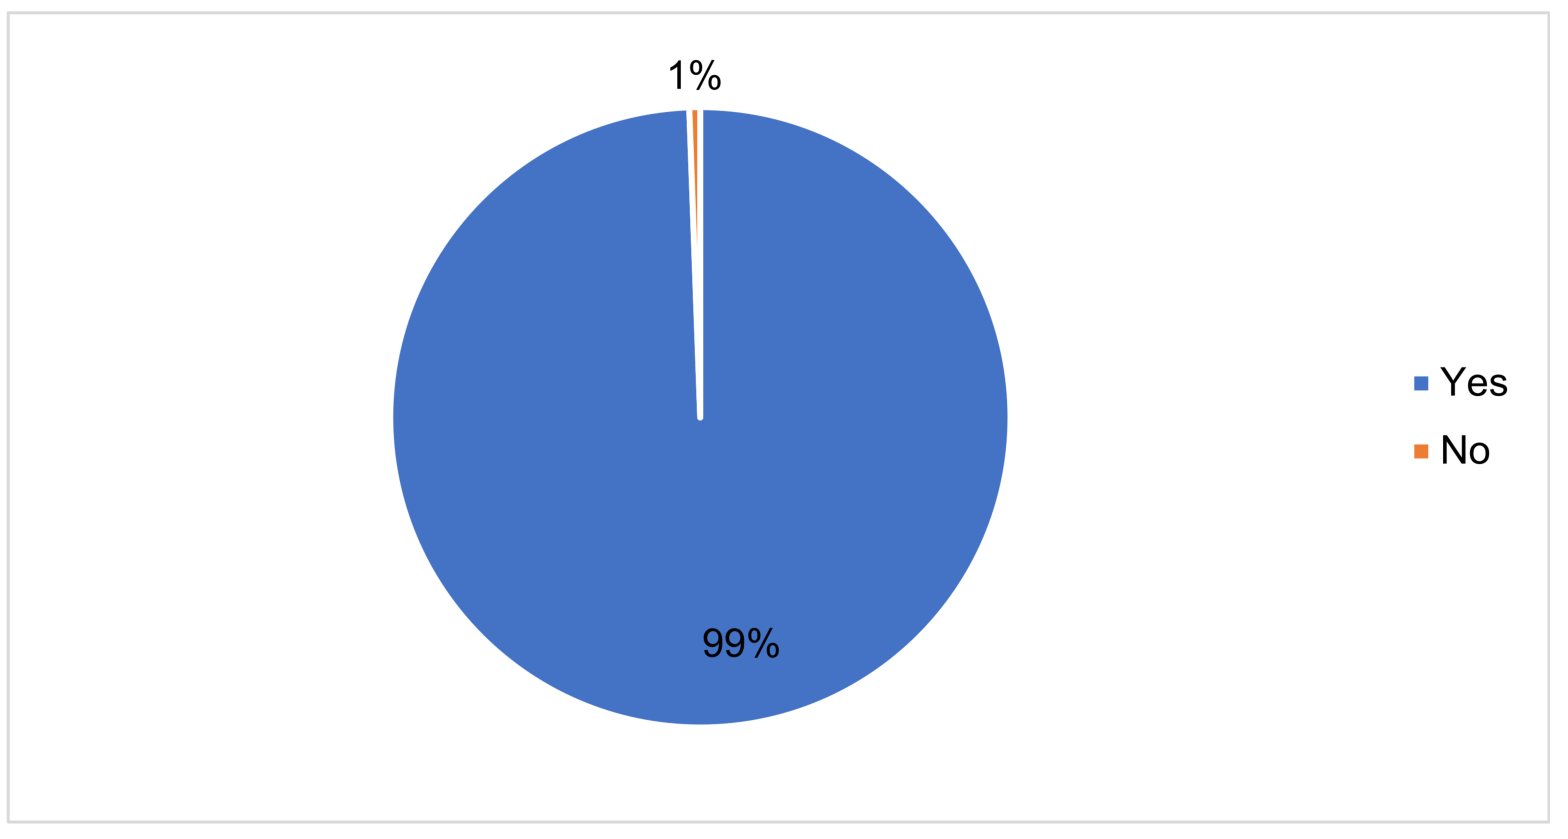
\includegraphics[width=\textwidth]{fig-012.pdf}
\caption{Do you think the UPEC must prepare an emergency plan to deal with an energy crisis in case power outages occur again in the future?}
\label{fig-12}
\source{Own elaboration based on the results of the survey administered in February 2025.}
\end{minipage}
\end{figure}

Finally, \Cref{fig-12} shows that 99\% of respondents indicated that UPEC should prepare an emergency plan to address future energy crises, whereas 1\% expressed a different view. This distribution reflects a broad agreement within the surveyed group regarding the importance of institutional preparedness in the event of future electricity interruptions. The marked concentration in the affirmative response highlights the perceived relevance of preventive planning among participants.

\section{Discussion}\label{sec-formato}
The power outages during the final quarter of 2024 significantly constrained hybrid education at UPEC. This imbalance carries profound digital-energy implications that extend beyond the mere interruption of classes. As \textcite{bacich2018metodologias} argue, while hybrid models are designed to offer flexibility and innovation, their sustainability is structurally dependent on an invisible yet vital infrastructure. When electricity fails, the ubiquity of communication—defined by \textcite{santaella2013comunicacao} as the ability to be present in any space-time—is disrupted, forcing students back into the physical and digital isolation that the hybrid model was intended to overcome.

In this context, it is crucial to recognize the response of the teaching staff, who navigated an unprecedented situation in which Ecuador accumulated 891 hours without electricity in 2024 \cite{eluniverso2024sinluz}. Such a scenario required rapid pedagogical adjustments and highlighted the structural vulnerability of technologically mediated educational models in contexts of energy instability.

One of the study’s most critical findings concerns the unequal capacity to sustain academic continuity. This situation reflects what \textcite{behar2020ensino} characterizes as the fragility of emergency remote teaching. While many students relied on mobile data or portable power sources, these solutions transferred the burden of adaptation onto the individual. Rather than functioning as collective safeguards, these strategies represented a form of privatized resilience, where academic continuity depended on personal resources. As \textcite{selwyn2017educacao} notes, digital inclusion often masks underlying material and socioeconomic disparities. The present findings reinforce this perspective, suggesting that energy crises do not merely interrupt educational processes but expose and potentially deepen structural inequalities.

Furthermore, this situation intersects with pre-existing structural challenges in higher education. Rising university dropout rates in Ecuador \cite{delgado2024desercion} provide a broader context in which energy instability acts as an additional stressor. Although most students did not report a high likelihood of withdrawal, a minority perceived a significant risk, indicating that prolonged infrastructural disruptions can exacerbate educational vulnerability. This confirms that without energy-resilient strategies, the hybrid model can inadvertently become a tool for exclusion rather than inclusion.

From an institutional standpoint, these findings underscore the necessity of proactive contingency planning. The near-unanimous support for an emergency plan reflects a collective recognition that hybrid education cannot rely solely on technological mediation without ensuring stable energy conditions. UPEC and similar higher education institutions must transition from a passive reliance on technology toward an active stance on technological sovereignty and crisis preparedness. In this sense, guaranteeing access to reliable electricity emerges not merely as an operational concern, but as a foundational requirement for educational equity and continuity in digitally mediated learning environments.


\section{Conclusion}\label{sec-modelo}
This study helped to evidence that the power outages registered in the last quarter of 2024 generated interruptions in the academic dynamics of UPEC students and deepened inequalities in terms of access to educational resources and adaptive capacity.

The intermittent power supply not only affected connectivity and participation in synchronous activities but also deteriorated study conditions, limiting the continuity of learning and compromising the academic performance of part of the student body.

This phenomenon underscores the need to guarantee emergent learning conditions, even in adverse scenarios, and highlights the crucial role that higher education institutions must play in the formulation of preventive and immediate response policies.

The fact that a considerable proportion of students considered abandoning their studies due to the crisis is evidence of the uncertainty caused by the absence of adequate conditions for their education.

The higher education system in Ecuador was already facing challenges in terms of student desertion, with rates that showed a worrying lack of academic continuity. The energy crisis was added to this structural problem, deepening even more the difficulties of permanence and student performance.

In this sense, it was corroborated that the energy crisis should be analyzed beyond a series of infrastructure failures, as a multidimensional phenomenon that directly affects the academic trajectory of students.

The planning of institutional protocols for the management of crises will guarantee a structured and timely response that minimizes the impact on the student community.

The interruption of the electricity supply affected the dynamics of teaching and learning in the short term and raised questions about its medium and long-term repercussions, making it imperative to continue with future research that analyzes the cumulative effects of this crisis.

\printbibliography\label{sec-bib}
% if the text is not in Portuguese, it might be necessary to use the code below instead to print the correct ABNT abbreviations [s.n.], [s.l.]
%\begin{portuguese}
%\printbibliography[title={Bibliography}]
%\end{portuguese}


%full list: conceptualization,datacuration,formalanalysis,funding,investigation,methodology,projadm,resources,software,supervision,validation,visualization,writing,review
\begin{contributors}[sec-contributors]
\authorcontribution{Patricio Moreno-Gudiño}[conceptualization,methodology,validation,visualization,writing]
\authorcontribution{Diana Ruiz-Onofre}[conceptualization,investigation,resources,validation,review]
\end{contributors}

\begin{dataavailability}
\txtdataavailability{databody} % options: dataavailable, dataonly, databody, datanotav, nodata
\end{dataavailability}

\appendix 
\section{Annex}\label{apx-longtable}

Link to the survey: \url{https://forms.gle/6qMFhtWDWr5xBHwr5}.



\end{document}

